\todo[backgroundcolor=magenta]{SEC: Introduce Network Theory}
Networks in the technical sense are analogous to networks in the nontechnical sense - a collection of objects paired with a number of connections that can link any two objects. \emph{Networks: An Introduction} by \emph{Mark Newman} lists \emph{Technological Networks}, \emph{Social Networks}, \emph{Information Networks} and \emph{Biological Networks} as different systems that are modelled by the technical interpretation of a network.\cite[Contents]{newman10}. A brief example of a network would be something like the following: Imagine you and your friends are represented as dots (nodes or vertices) on a piece of paper. Then if any two people are friends, the dots representing those people are connected by a line (edge). If you then repeat this process by asking your friends to list all their friends and so on, you will end up with a simple model of a \emph{social network}.

As one might imagine, now that we have this model it's easy to be curious about any structure that emerges that we can detect and abuse to develop an understanding of the real world system that we are representing. The structure that this essay will explore is that of \emph{communities}. Vaguely speaking, communities are subsets of a network that are \emph{densely connected} amongst themselves. I.e. there is some notion of any node within a community being more closely connected to other nodes in the community than nodes outside the community in the average case. Before we dive into the details of communities and detecting them, I wish to provide some motivation by way of example of the kinds of situations that networks can arise and why they are the natural model for the related systems.

\subsection{Social Networks}\label{sec:Social Networks}
\todo[backgroundcolor=orange]{SEC: Models of Networks}
To better illustrate the simple notion of a social network mentioned above, I will introduce the canonical network theory example of \emph{Zachary's Karate Club}. Zachary's Karate Club is a dataset where "The data was collected from the members of a university karate club by Wayne Zachary in 1977.  Each node represents a member of the club, and each edge represents a tie between two members of the club."\cite[Metadata]{konect:2017:ucidata-zachary}\todo[backgroundcolor=yellow]{Am I supposed/allowed to reference like this?}. In Figure \ref{fig:zachary_digrams}, there are two different renderings of the Zachary Karate Club. Figure \ref{fig:zachary_spring} shows the network rendered using a "spring" layout (which is a type of force directed graph drawing\cite{kobourov12})and figure \ref{fig:zachary_circle} shows the network rendered using a "circle" layout. These different layouts show us different parts of the underlying structure of the network. \todo[backgroundcolor=yellow]{Should I include any code that I write too even if it's just a small example like this?}

\begin{figure}
    \begin{center}
        \begin{subfigure}[b]{0.45\textwidth}
            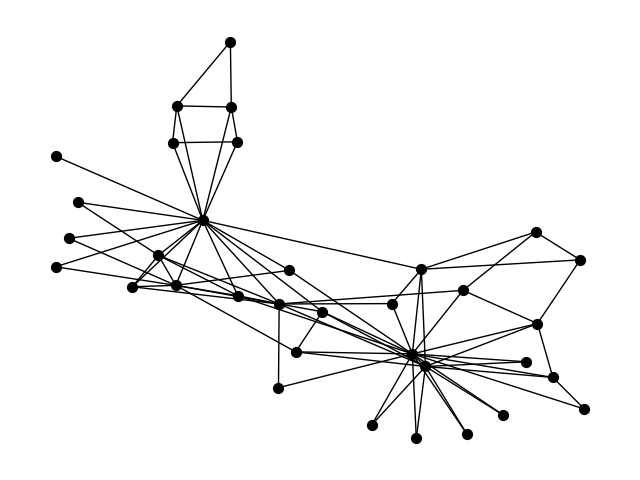
\includegraphics[width=\textwidth]{img/zachary_spring}
            \caption{Spring Layout}
            \label{fig:zachary_spring}
        \end{subfigure}
        \begin{subfigure}[b]{0.45\textwidth}
            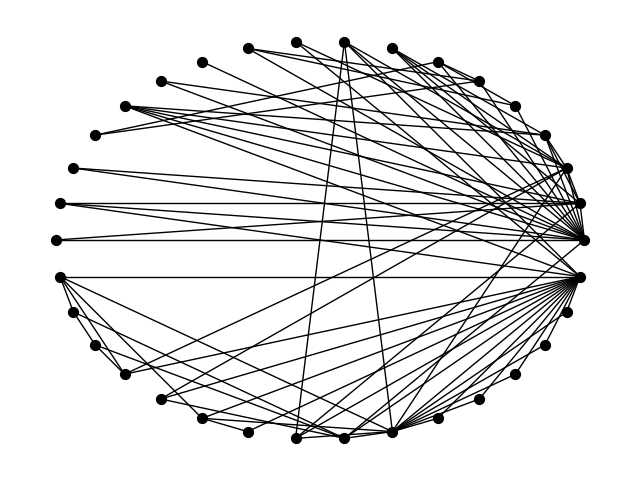
\includegraphics[width=\textwidth]{img/zachary_circle}
            \caption{Circle Layout}
            \label{fig:zachary_circle}
        \end{subfigure}
    \end{center}
    \caption{Two renderings of the Zachary Karate Club network using data from KONECT.cc\cite{konect:2017:ucidata-zachary} and a Python library NetworkX\cite{SciPyProceedings_11}}
    \label{fig:zachary_digrams}
\end{figure}

\subsection{Technological Networks}\label{sec:Technological Networks}
\subsection{Information Networks}\label{sec:Information Networks}
\subsection{Biological Networks}\label{sec:Biological Networks}

\todo[backgroundcolor=red]{SEC: Definition of a Network}
\todo[backgroundcolor=red]{SEC: Different Types of Network}
